\chapter{Methodik und Implementierung}
Dieses Kapitel führt das Vorgehen und die Implementierung eines C++ Programms aus, die es ermöglichen Aussagen über den Speicher des Kaffeevollautomaten zu treffen.
Immer wiederkehrende Arbeitsabläufe werden von diesem Programm übernommen und auf den unteren Ebenen automatisiert.

\section{Vorgehen}
Die Speicher des Kaffeevollautomaten, der \ac{EEPROM} und der \ac{RAM}, können Zeilenweise ausgelesen werden.
Der nötige Zugriff zum Auslesen kann auf zwei Arten erfolgen: direkt am Speicherstein auf der Hauptplatine oder seriell über die vorhandene \ac{UART} Schnittstelle, siehe Abschnitt~\ref{subsec:zugangSeriellDirekt}.
Im Folgenden erfolgt die Kommunikation über die \ac{UART} Schnittstelle und mithilfe der \textit{libserial}-Library.

Unabhängig voneinander wurden beide Speicher untersucht.
Ein eigens entwickeltes C++ Programm setzt die sechzehn Zeilen einer Speicherabfrage zu einem gesamten Speicherauszug zusammen.
Intern werden dabei je zwei Hexadezimalzahlen in eine ganzzahlige Dezimalzahl umgerechnet und in einem Vektor abgelegt.
Dadurch sind Position und Wert bekannt.

\begin{figure}
  \begin{center}
    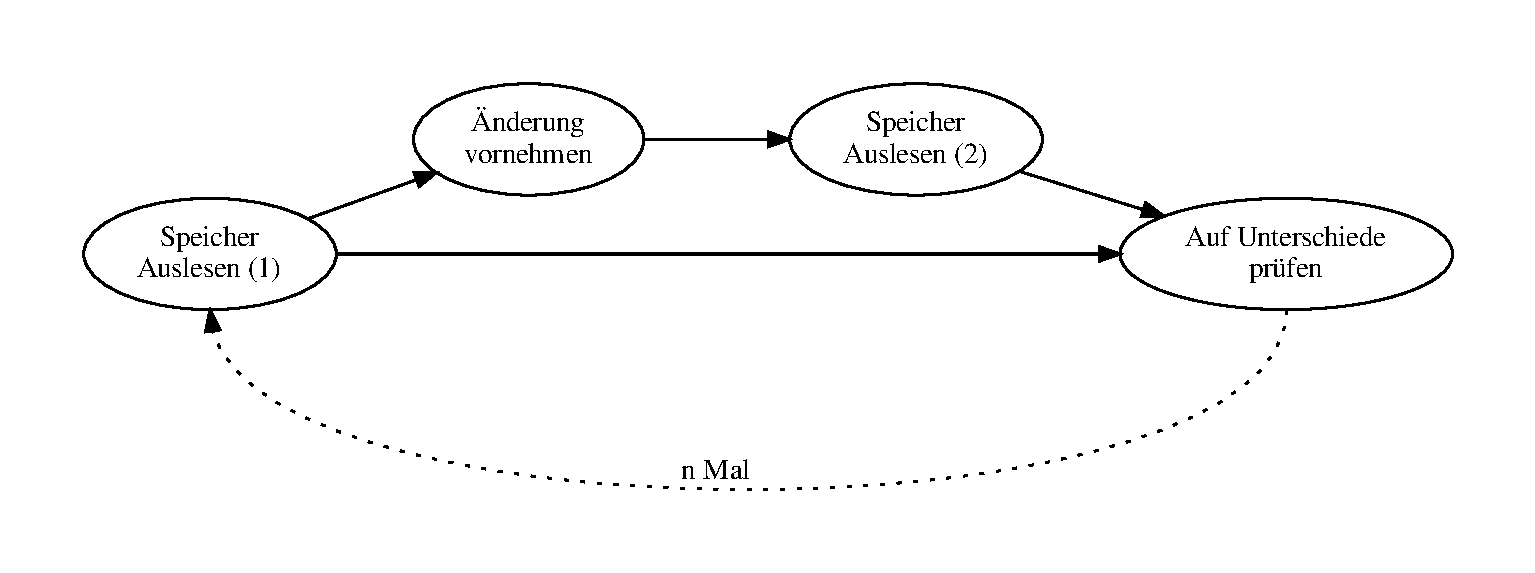
\includegraphics[scale=0.54]{images/chapter_4/workflow}
    \caption{Arbeitsablauf}
    \label{fig:workflow}
  \end{center}
\end{figure}

Abbildung~\ref{fig:workflow} visualisiert den Arbeitsablauf der zur Bestimmung der Speicherstellen in dieser Arbeit angewandt wurde.
Nach dem ersten Schritt ganz links wird nun von Hand eine möglichst elementare Veränderung an dem Kaffeevollautomaten vorgenommen, um gezielten Aktionen die Werteänderungen bestimmter Speicherzellen zuordnen zu können.
Die angewandten Veränderungen werden in Abschnitt~\ref{subsec:AenderungenAnDerMaschine} beschrieben.

Nach einer erneuten Aufnahme eines Speicherauszugs können diese beiden nun verglichen werden.
Das Programm iteriert durch den Vektor und vergleicht die Speicherwerte an der gleichen Position.
Bei Ungleichheit existiert ein Unterschied der festgehalten wird.
Dieser Ablauf wurde auf alle Einstellmöglichkeiten und Funktionen des Kaffeevollautomaten angewandt.

Bei dem \ac{RAM}, im Gegensatz zum \ac{EEPROM}, fiel jedoch auf, dass sich mehrere Speicherwerte auch ohne eine vorgenommene Veränderung änderten.
Deshalb wurden viele Speicherauszüge im Ruhezustand aufgenommen und die sich regelmäßig ändernden Bytes ausgeschlossen.
Zu Beginn der Ergebnisse über den \ac{RAM} in Abschnitt~\ref{sec:ErgebnisseRAM} sind diese aufgeführt.
Dennoch gab es gelegentliche Unregelmäßigkeiten, sodass das Vorgehen für den \ac{RAM} um eine geschlossene Rückrichtung ergänzt wurde.
In der Regel wurden pro \ac{RAM} Funktion $n=3$ Durchläufe vorgenommen und die gemeinsame Schnittmenge der Veränderungen bestimmt.

Ganz am Ende gab es noch ein zweites Vorgehen, bei dem gezielt der \ac{EEPROM} an bekannten Speicherstellen beschrieben wurde.
Hintergrund war die unbekannte Position bzw. später die Zusammensetzung des Bezüge-Zählers im Einstellungsmenü des Kaffeevollautomaten.
Abschnitt~\ref{subsec:Vorgehen2} führt dies im Folgenden aus.

\subsection{Veränderungen zur Bestimmung der Speicherstellen}\label{subsec:AenderungenAnDerMaschine}
\subfigbox{
  \subfigure[Fassung im Kaffeevollautomaten]{\label{subfig:fassung}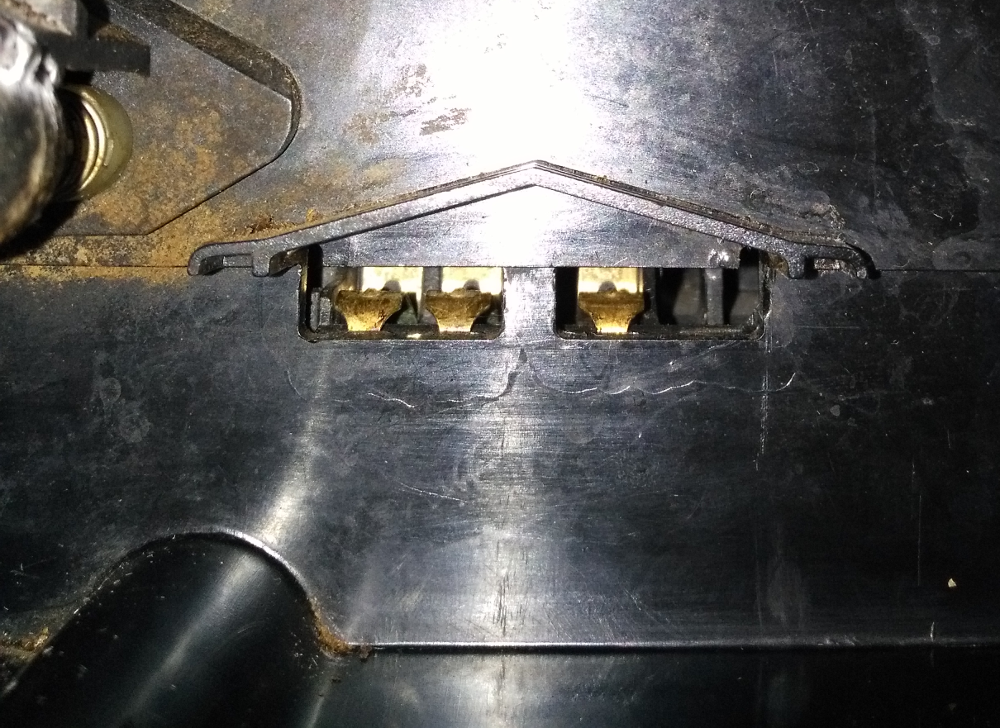
\includegraphics[scale=0.2]{images/chapter_4/Schale-Fassung}}\\%
  \subfigure[Oberseite des Schalen Ersatzes]{\label{subfig:oberseite}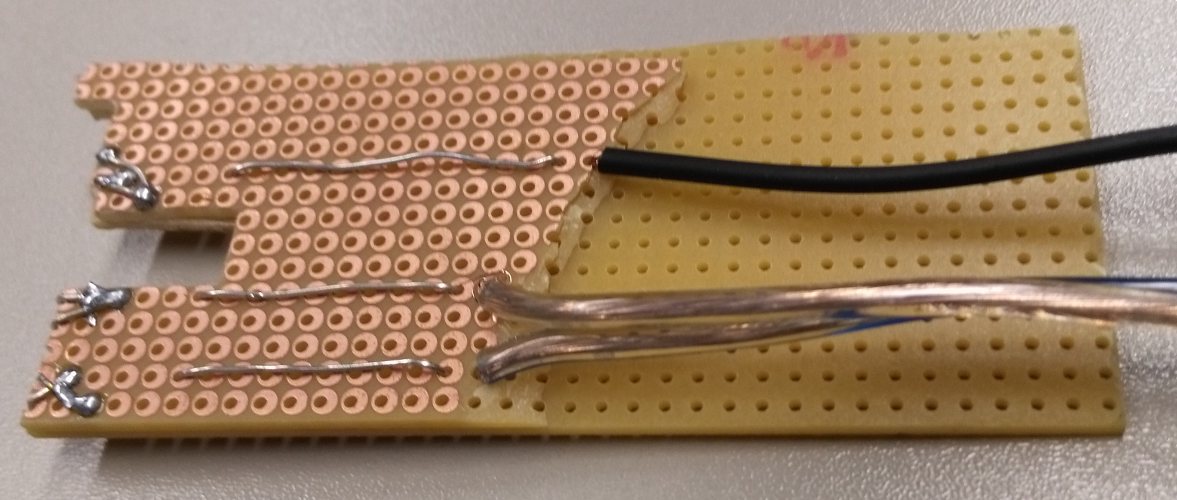
\includegraphics[scale=0.29]{images/chapter_4/Schale-Oberseite}}\\%
  \subfigure[Unterseite des Schalen Ersatzes]{\label{subfig:unterseite}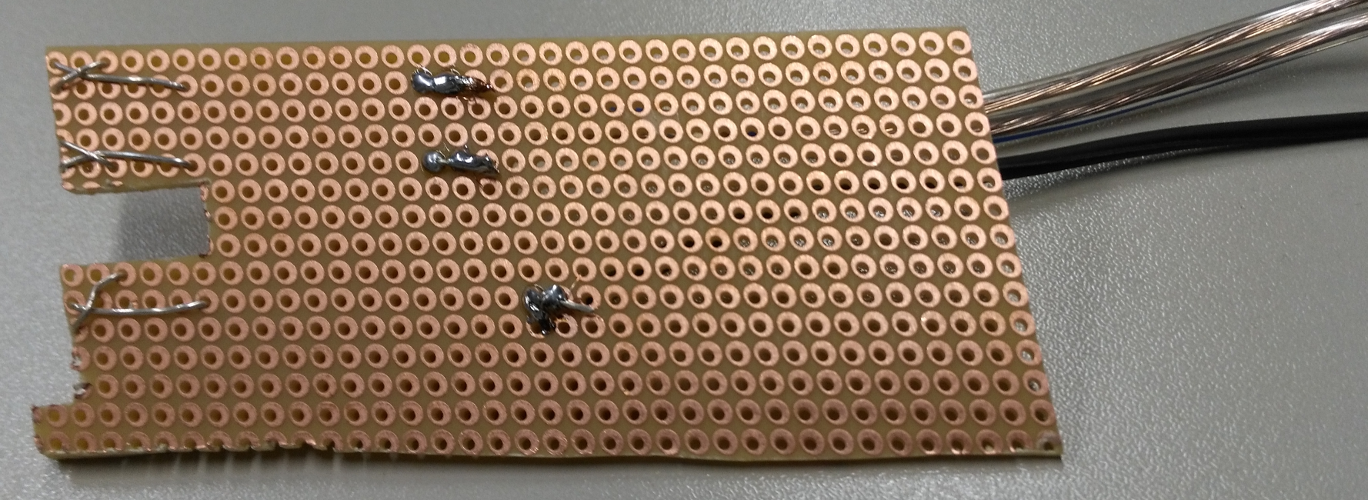
\includegraphics[scale=0.25]{images/chapter_4/Schale-Unterseite}}%
}{Ersatz der Schale des Kaffeevollautomaten}{fig:ersatzschale}

Für den \ac{EEPROM} war es hilfreich einmal das Handbuch der Maschine systematisch durch zugehen und zum Beispiel immer eine Menüoption zu variieren.
Bei einer Skala (wie z.B. beim Kaffeepulver) hat es ausgereicht den niedrigsten, den höchsten und den Standard-Wert im Speicher zu bestimmen;
deckte sich die einstellbare Anzahl an Abstufungen mit der Werte Differenz im Speicher, ließ sich auf die verbleibenden Werte schließen.
Auch im normalen Gebrauch fiel somit u.a. ein Einschaltzähler im \ac{EEPROM} auf.

Für den \ac{RAM} ging es mit den gezielt auslösbaren Statusmeldungen los.
Das Anheben des Wassertanks oder das Abziehen der unteren Schale löste eine Warnmeldung auf dem Display aus und wurde auch im \ac{RAM} vermerkt.
Ein zu hoher Wasserstand in der Schale konnte ohne Wasser mit einer eigenen Platine vorgegaukelt werden.
Abbildung~\ref{subfig:fassung} zeigt die Fassung an der Rückwand innerhalb des Kaffeevollautomaten für die Schale.
Abbildung~\ref{subfig:oberseite} und \ref{subfig:unterseite} visualisieren die Platine, an der leicht von außen mittels Krokodilklemmen die Kontakte im Inneren kurzgeschlossen werden konnten.
Am schwierigsten sind komplexe Abläufe, wie die Zubereitung eines Kaffees.
Hier konnte nur mehrfach zu gezielt gleichen oder ungleichen Zeitabständen der zweite Speicherauszug angestoßen werden.
Hier sei schon einmal der Verweis auf Abschnitt~\ref{sec:AussagekraftDerErgebnisse} zur Aussagekraft dieser Ergebnisse genannt worden.

Abschließend war auch für das Display ein kleines Programm nötig um die volle Funktionsvielfalt festzustellen.
Abschnitt~\ref{subsec:tools} führt dies später aus.

\subsection{EEPROM gezielt beschreiben}\label{subsec:Vorgehen2}
Ziel war es die unbekannte Position bzw. später die Zusammensetzung des Bezüge-Zählers im Einstellungsmenü des Kaffeevollautomaten zu entziffern.
Dafür wurde die angezeigt Zahl in eine Hexadezimalzahl umgerechnet und im Speicherauszug des \ac{EEPROM} des Kaffeevollautomaten gesucht.
Da die Zahl eine Stromunterbrechung überstand und eine Änderung des einzigen übereinstimmenden Wertependants in Wort \wort{15} keine Änderung der Ausgabe hervorrief, begann die Suche an weiteren bekannten Speicherstellen im \ac{EEPROM}.

Der Bezüge-Zähler setzt sich aus mehreren Zählern zusammen.
Der Trester Füllstand in der Schale wird nicht gemessen, sondern im Betrieb gezählt um den Füllstand zu erfassen.
Auch die Reinigungsankündigung beruht auf Zählständen über Kaffee Bezüge und Spülungen.
Die Wasser Durchflussmenge des Filters wird ebenfalls erfasst und ab einem festen Wert eine Warnmeldung zum Wechseln ausgegeben.

Das gezielte eingreifen in die Zählstände ließ es zu diese Grenzwerte zu bestimmen.
Die Ergebnisse befinden sich in Abschnitt~\ref{subsec:ErgebnisKaffeezubereitung}.

\section{Das C++ Programm "`./JuraCoffeeMemory"'}
Für diese Arbeit wurde ein C++ Programm entwickelt, das die Kommunikation und die Aufschlüsselung der Antworten übernommen hat.

\subsection{Makefile}
In dem Projekt Ordner befinden sich auf der Hauptebene mehrere \texttt{CPP}- und \texttt{HPP}-, eine \texttt{H}- sowie eine \texttt{Makefile}-Datei.
Sind die in der \texttt{Readme.md} genannten Abhängigkeiten und Voraussetzungen erfüllt, kann das Projekt mit dem Befehl \texttt{make}, ohne Zusatzangaben gebaut werden.
Am Ende sollte dann auf der Hauptebene eine ausführbare Datei namens \texttt{./JuraCoffeeMemory} herauskommen.
Es werden neben Objekt-Dateien auch noch einige weitere Tools im Unterordner \texttt{./tools/} gebaut, auf die später in Abschnitt~\ref{subsec:tools} eingegangen wird.

Der Befehl \texttt{make clean} entfernt die Objekt-Dateien, mittels \texttt{make dist-clean} werden ebenfalls die ausführbaren Programme entfernt und der Projekt Ordner in seinen Ursprungszustand zurück versetzt.

\subsection{Interaktives Menü}
Startet man in einem Terminal das Hauptprogramm \texttt{./JuraCoffeeMemory} wird das Hauptmenü angezeigt. Abbildung~\ref{subfig:terminal1-MainMenu} visualisiert diesen Zustand.
Das Listing~\ref{lst:menu-tree} zeigt einmal schematisch all Menüoptionen.

\subfigbox{
  \subfigure[Hauptmenü]{\label{subfig:terminal1-MainMenu}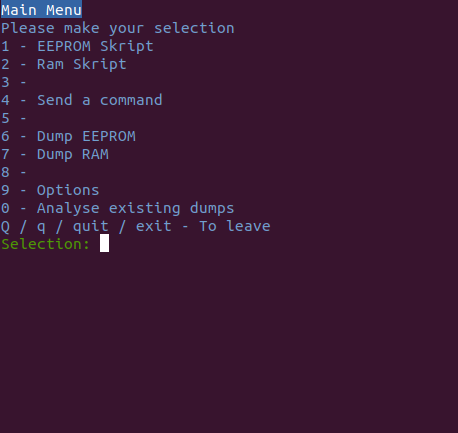
\includegraphics[scale=0.4]{images/chapter_4/JuraCoffeeMemory-1-MainMenu}}\hfill%
  \subfigure[Optionen $\leadsto$ Log Pfad ändern]{\label{subfig:terminal7-Options-RamLogFilePath}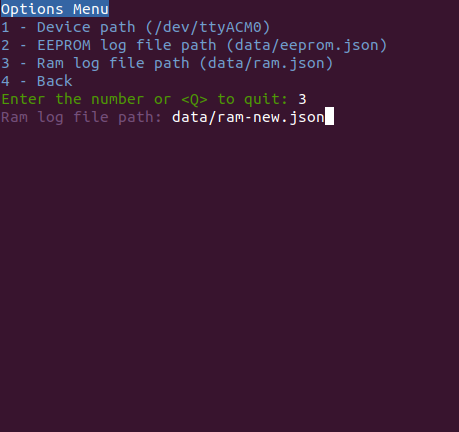
\includegraphics[scale=0.4]{images/chapter_4/JuraCoffeeMemory-7-Options-RamLogFilePath}}\\%
  \subfigure[RAM Speicherauszug]{\label{subfig:terminal5-RAM-dump}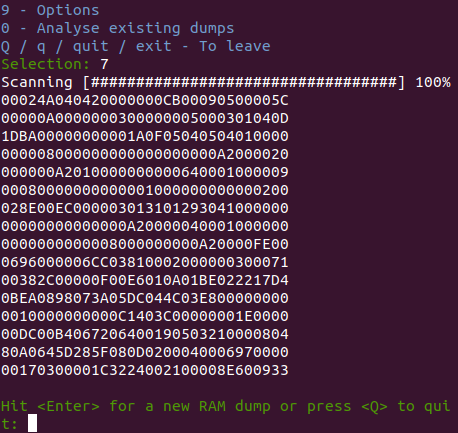
\includegraphics[scale=0.4]{images/chapter_4/JuraCoffeeMemory-5-RAM-dump}}\hfill%
  \subfigure[EEPROM Skript]{\label{subfig:terminal3-EEPROM-NothingChanged}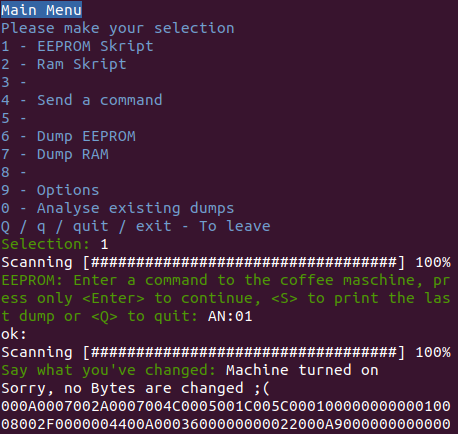
\includegraphics[scale=0.4]{images/chapter_4/JuraCoffeeMemory-3-EEPROM-NothingChanged}}\\%
%  \subfigure[Befehl senden]{\label{subfig:terminal4-Send-TY}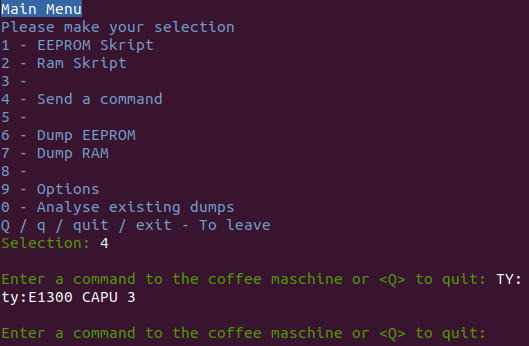
\includegraphics[scale=0.4]{images/chapter_4/JuraCoffeeMemory-4-Send-TY}}%
  \subfigure[Auswertungen]{\label{subfig:terminal8-AnalyseDumpsMenu}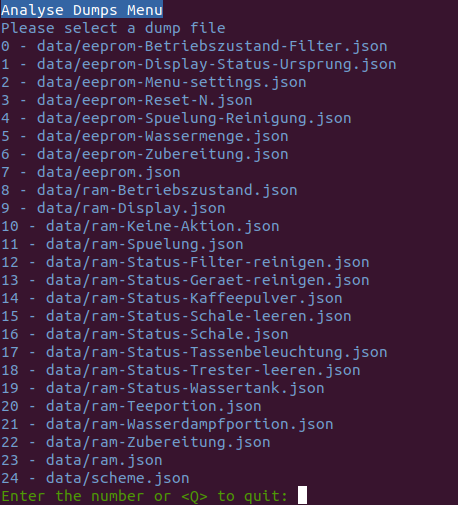
\includegraphics[scale=0.3]{images/chapter_4/JuraCoffeeMemory-8-AnalyseDumpsMenu}}\hfill%
  \subfigure[Speicherauszug einsehen]{\label{subfig:terminal9-AnalyseFilterDump}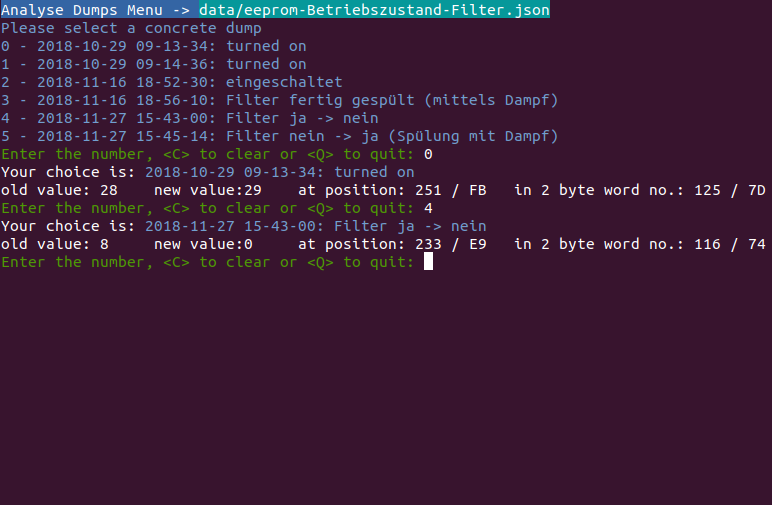
\includegraphics[scale=0.3]{images/chapter_4/JuraCoffeeMemory-9-AnalyseFilterDump}}%
}{Interaktives Menü des C++ Programms "`./JuraCoffeeMemory"'}{fig:terminal}

\begin{lstlisting}[label=lst:menu-tree,caption={Menü-Baum ./JuraCoffeeMemory}]
Main Menu
|-- 1: EEPROM Skript
|-- 2: Ram Skript
|-- 4: Send a command
|-- 6: Dump EEPROM
|-- 7: Dump RAM
|-- 9: Options
|   |-- 1: Device path (/dev/ttyACM0)
|   |-- 2: EEPROM log file path (data/eeprom.json)
|   |-- 3: Ram log file path (data/ram.json)
|   `-- 4: Back
|-- 0: Analyse existing dumps
|   |-- Analyse Dumps Menu
|   |   |-- data/xxx.json
|   |   |   `-- Dumps
|   |   |-- C: Clear window
|   |   `-- Q: Quit
|   `-- Q: Quit
`-- Q / q / quit / exit: To leave
\end{lstlisting}

\todo
Abbildung~\ref{subfig:terminal7-Options-RamLogFilePath}
Abbildung~\ref{subfig:terminal5-RAM-dump}
Abbildung~\ref{subfig:terminal3-EEPROM-NothingChanged}
Abbildung~\ref{subfig:terminal8-AnalyseDumpsMenu}
Abbildung~\ref{subfig:terminal9-AnalyseFilterDump}
\todo ...

\subsubsection{Farbcodierungen}
Normale Ausgaben sowie Benutzer Eingaben erscheinen in weißer Schrift.
Weiße Schrift auf blauem Grund stellt Menü Überschriften dar.
In blauer Schrift sind Menüs dargestellt.
Grüne Schrift vor der blinkenden Eingabemarke fordert zur Eingabe auf.
Der Text beschreibt valide Eingaben.
Abschließend beschreibt roter Text einen Fehler.
Die aufgetretene Position wird in weißer Schrift auf rotem Grund hervorgehoben.

\subsection{Die API nach außen}
Das Hauptprogramm kann aber auch über vier Parameter aufgerufen werden. Die Ausgaben sind dann im fehlerfreien Fall farblose \ac{JSON} Zeichenketten oder einfacher Text in die Standardausgabe.

Mögliche Fehlermeldungen sind für Entwickler in der \texttt{Readme.md} dokumentiert.
Die Fehler Ausgabe erfolgt wie im interaktiven Menü mit Farben.
Für Entwickler bietet sich daher der Rückgabewert des Programms an.

\paragraph{./JuraCoffeeMemory command}
Von der Standardeingabe wird eine Zeichenkette erwartet, die an den Kaffeevollautomaten weiter gegeben wird.
Mögliche Eingaben sind die Befehle aus der Tabelle~\ref{tbl:kommandos}.
Die Antwort des Kaffeevollautomaten erscheint als einfacher Text.

\paragraph{./JuraCoffeeMemory eepromWrite}
Bei diesem Aufruf wird von der Standardeingabe ein \ac{JSON} Objekt erwartet.
Alle dort genannten Bezeichnungen werden abgearbeitet und die neuen Werte im Speicher des Kaffeevollautomaten hinterlegt.
Auf der obersten Ebene müssen sich aus \texttt{EEPROM\_Status::getEntriesEEPROM()} bekannte Bezeichnungen befinden, die ein Unterobjekt mit der Bezeichnung \texttt{value} sowie je einem ganzzahligen Wert beinhalten.
Listing~\ref{lst:eepromWrite} veranschaulicht dies an einem Beispiel.

Treffen die Bedingungen zu, wird ein Schreib-Befehl an den Kaffeevollautomaten gesandt.
Die Antworten werden in einer Zeichenkette mit der verwendeten Bezeichnung und dem Text "`\#\#\#"' als Abstandshalter festgehalten und auf der Standardausgabe ausgegeben.
Die Antwort auf das Beispiel Listing~\ref{lst:eepromWrite} steht in Listing~\ref{lst:eepromWriteAnswer}.

\begin{lstlisting}[label=lst:eepromWrite,caption={Beispiel einer JSON Eingabe für./JuraCoffeeMemory eepromWrite}]
{
  "powder_quantity_special_coffee": {
    "value": 11
  },
  "water_quantity_special_coffee": {
    "value":  380
  }
}
\end{lstlisting}

\begin{lstlisting}[label=lst:eepromWriteAnswer,caption={Antwort auf das Beispiel der JSON Eingabe}]
ok: powder_quantity_special_coffee###ok: water_quantity_special_coffee###
\end{lstlisting}

\paragraph{./JuraCoffeeMemory eeprom}
Nach ungefähr fünf Sekunden erhält man die aktuellen Einstellungen und Zählstände des \ac{EEPROM} in einem kompakten \ac{JSON} Objekt.
Im Gegensatz zum EEPROM Skript werden nur die nötigen Speicherstellen abgefragt.
Die Bezeichnung der Speicherstellen, die auch der Name eines \ac{JSON} Eintrags ist, befindet sich mit der zugehörigen Adresse in \texttt{EEPROM\_Status::getEntriesEEPROM()}.
Eine Adresse besteht aus der Position eines Wortes sowie einer oder beider Bytes.
Von Hand sind dort zum Teil weitere Hintergrundinformationen, wie Standardwerte über die \texttt{[N]}-Taste des Kaffeevollautomaten, minimale und maximale Schranken, der Wert für einen deaktivierten Zustand oder überhaupt ausschließlich zugelassene Werte hinterlegt.

\paragraph{./JuraCoffeeMemory ram}
Ähnlich zum Abfragen des \ac{EEPROM} wird hier aber der \ac{RAM} in ungefähr drei Sekunden an den entscheidenden Stellen ausgelesen.
Die Assoziation einer Bezeichnung mit ihrer Speicherposition geschieht in \texttt{RAM\_Status::getEntriesRAM()}.
Hier wird ein Byte und ggf. mehrere zusammenhängende Bits als ein Eintrag abgelegt.
Als Ausgabe erfolgt ein kompaktes \ac{JSON} Objekt.










\subsection{Zugrunde liegende Klassenstruktur}

\subsection{...}\todo



% $ ll *.cpp
% EEPROM.cpp
% EEPROM_Status.cpp
% JsonFile.cpp
% JuraCoffeeMemory.cpp
% RAM.cpp
% RAM_Status.cpp
% SerialConnection.cpp
% Storage.cpp

% $ ll *.h*
% color-definitions.h
% EEPROM.hpp
% EEPROM\_Status.hpp
% JsonFile.hpp
% RAM.hpp
% RAM\_Status.hpp
% SerialConnection.hpp
% Storage.hpp

\todo

% ./RAM.cpp
% ./JsonFile.cpp
% ./Storage.cpp
% ./JuraCoffeeMemory.cpp
% ./tools/libserial-test/main.cpp
% ./tools/display.cpp
% ./tools/formate-dump.cpp
% ./tools/jsoncpp-test/main.cpp
% ./tools/display-screen-saver.cpp
% ./tools/Ideen/Ctrl-D\_stop.cpp
% ./tools/Ideen/byte-bit.cpp
% ./tools/Ideen/progressbar.cpp
% ./tools/Ideen/byte-bit-2.cpp
% ./tools/Ideen/lock-file.cpp
% ./RAM\_Status.cpp
% ./EEPROM.cpp
% ./EEPROM\_Status.cpp
% ./SerialConnection.cpp


\section{Weitere kleine Tools}\label{subsec:tools}
Im Unterordner \texttt{./tools/} befinden sich nach dem Aufruf von \texttt{make} drei kleine Programme.

\subsection{Formatieren eines Speicherauszugs}
Ruf man \texttt{./tools/formate-dump} auf, kann man dem Programm eine Zeichenkette aus $1024$ oder $512$ Hexadezimalzeichen übergeben.
Das Programm erkennt an der Größe \ac{EEPROM} und \ac{RAM} Eingaben und wertet den Speicherauszug um Angaben wie die Speicherposition und Dezimal-/Hexadezimalzahlen Formate auf.

\subsection{Display}
Um den verfügbaren Zeichensatz des Displays in der oberen linken Ecke an der Front des Kaffeevollautomaten zu bestimmen, wurde ein kleines Extraprogramm entwickelt.
Anlass waren Sonderzeichen und die deutschen Umlaute, die sich über die gegebenen Befehle (\texttt{?D0}, \texttt{?D1xxx}, \texttt{?D2xxx}) nicht einfach auf das Display bringen ließen.
Das Programm \texttt{./tools/display} iterierte einmal systematisch über die Zahlen von $0$ bis ungefähr $260$ und gab einen Befehl zum Anzeigen der Dezimalzahl sowie des dazugehörigen \ac{ASCII}-Zeichens an den Kaffeevollautomaten.
Dies umfasst das einfache und erweiterte \ac{ASCII} Alphabet sowie einige weitere Zahlen bzw. Zeichen.
Dabei stellte sich nur ein mittlerer Block des einfachen \ac{ASCII}-Alphabets als interessant heraus, der jetzt eingegrenzt von eben diesem Programm durchlaufen wird.
Ein weiteres Programm namens \texttt{./tools/display-screen-saver} veranschaulicht die damit verbundenen Möglichkeiten.

Die gegebenen Befehle über die serielle Verbindung \texttt{?D0}, \texttt{?D1xxx} und \texttt{?D2xxx} verändern nur den Standardtext "`Kaffee bereit"'.
Andere Texte, wie das Programmmenü oder Warnmeldungen, überlagern den Standardtext mit den einprogrammierten Texten aus den vorhandenen Sprachen.

Möchte man die Ausgaben des ersten Programms nachstellen ist zu beachten, dass der Kaffeevollautomat eingeschaltet sein muss und auch an die erste Displayzeile ein Ausgabebefehl gegangen ist, damit die Ausgabe auch sichtbar wird.
Das Programm verändert dann die zweite Zeile.
Folgende Befehlseingaben werden empfohlen:
\begin{enumerate}
  \item \texttt{cd JuraCoffeeMemory/}
  \item \texttt{make}
  \item \texttt{./JuraCoffeeMemory}
  \item \texttt{4} (Senden eines Kommandos)
  \item \texttt{AN:01} (Maschine einschalten)
  \item \texttt{?D1xxx} (Etwas Text an die erste Displayzeile)
  \item \texttt{<Strg>+D} (Verlassen des Programms)
  \item \texttt{./tools/display}
\end{enumerate}

\section{Die Webseite}

Die Webseite ist zu sehen in Abbildung~\ref{fig:website}.
Nach ein paar Hinweisen kann im oberen Bereich der einzelne Kaffee sowie die gesamte Maschine konfiguriert werden.
Für jede Kaffeeart ist es möglich sich seine eigene Konfiguration in einem lokalen Webbrowser-Keks (Cookie) abzuspeichern und komfortabel in den Speicher des Kaffeevollautomaten zu schreiben um sich anschließend einen Kaffee zubereiten zu lassen.
Der Keks kann auch wieder entfernt werden oder sich auf die Standardwerte zurücksetzen lassen.
Prinzipiell kann hierüber der ganze bekannte \ac{EEPROM} überschrieben werden.

Im nächsten Absatz sind Statusinformationen aus dem \ac{RAM} einsehbar.
Einige Meldungen werden am Bild des Kaffeevollautomaten visualisiert.
Der Status kann über \texttt{Refresh} aktualisiert werden.
Einfache "`ja"' oder "`nein"' Meldungen werden durch eine grünes "`on"' oder rotes "`off"' präsentiert.
Informationen, die sich über mehrere Bits erstrecken werden mit ihrem entsprechenden Zahlenwert dargestellt.

Im letzten Abschnitt befinden sich Zählstände und Prozent-Anzeigen, die verdeutlichen wie weit es noch bis zur nächsten Warnmeldung, wie Trester leeren, Maschine reinigen oder Filter wechseln, ist.

Wenn am Computer der Mauszeiger auf einer Zahl oder Einstellung zum Finger wird, öffnet sich mit einem Klick ein Fenster, in dem der Wert verändert werden kann.
Nach Möglichkeit werden der Standardwert, der Wert zum Deaktivieren und weitere Hinweis Texte angeboten.

Unten rechts auf der Seite kann über \texttt{Command} ein Kommando aus der Tabelle~\ref{tbl:kommandos} an den Kaffeevollautomaten abgesetzt werden.
Eine Liste bietet viele Vorschläge mit dazugehörigen Bezeichnungen.
Recht daneben aktualisiert ein Klick auf \texttt{Refresh} die Statusinformationen aus dem \ac{RAM}.
Ganz rechts in der Ecke kann eine Tour durch die Bedienung der Seite gestartet werden.

\begin{figure}
  \begin{center}
    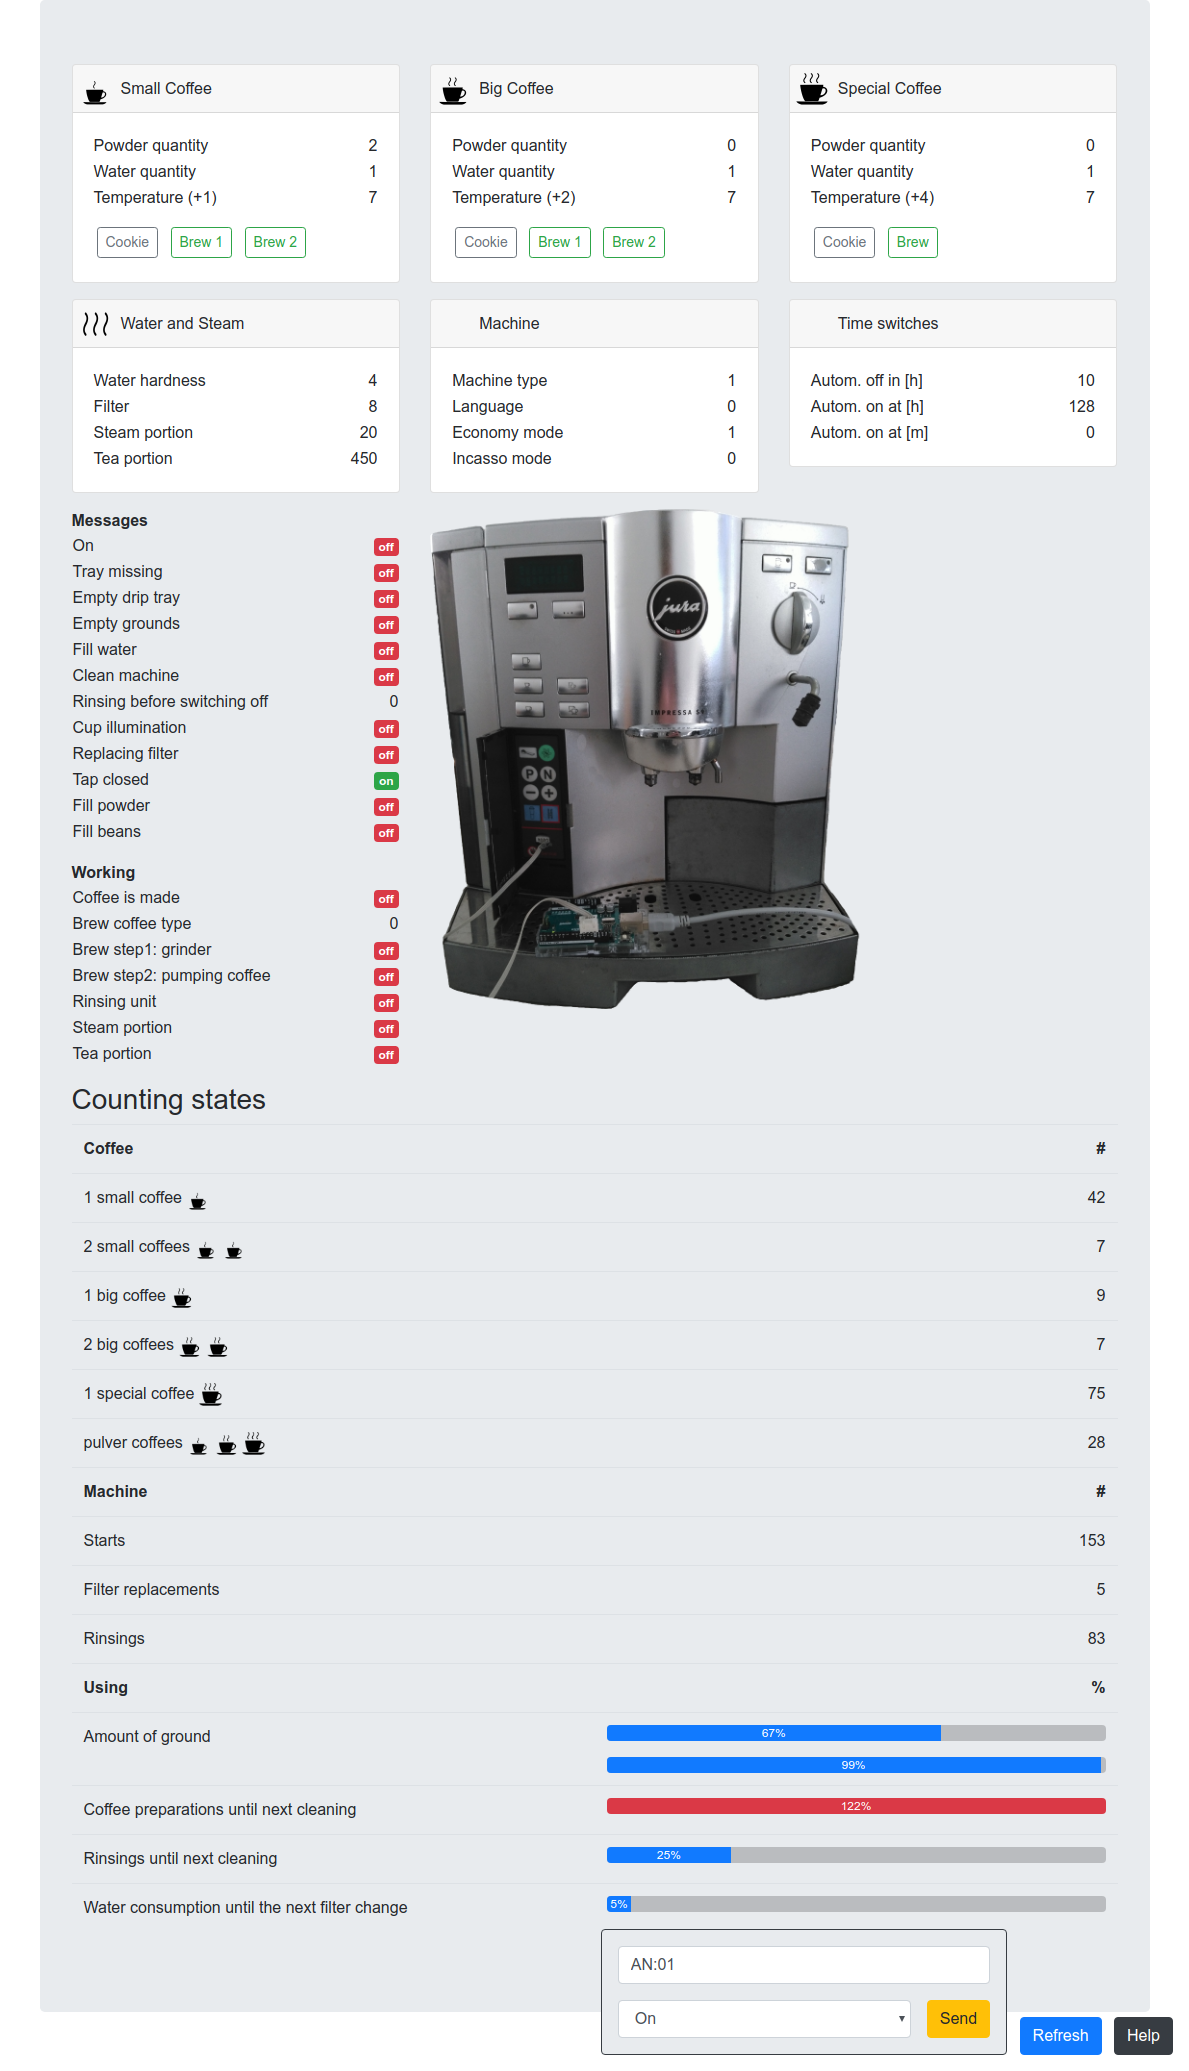
\includegraphics[scale=0.25]{images/chapter_4/Webseite}
    \caption{Die Webseite}
    \label{fig:website}
  \end{center}
\end{figure}

\subsection{Die technische Umsetzung}
Die Webseite befindet sich im Projektunterordner \texttt{./website/}.
Die Datei \texttt{data.php} nimmt Parameter entgegen und ruft damit das C++ Programm mit evtl. Datenübergaben auf.
Die Antwort des C++ Programms wird in einem \ac{JSON}-Objekt verpackt und der Webseite zurück gegeben.
Bei Problemen wird aber auch die Fehlernummer (der Rückgabewert des Programms) einschließlich der Meldung leicht zugänglich in einem \ac{JSON}-Objekt zurück gegeben.

Die für den Benutzer ersichtliche Webseite besteht primär aus den Dateien \texttt{index.html}, \texttt{script.js} für die Interaktion und \texttt{style.css} für das individuelle Layout.
Weitere eingebundene Dateien sind das Favicon im Unterordner \texttt{favicon/}, Bilder im Unterordner \texttt{img/}, \texttt{intro.min.js} und \texttt{intro.min.css} für die Tour durch die Webseite, \texttt{offline\_eeprom.json} und \texttt{offline\_ram.json} für die Offline-Funktion, in der die Webseite ersichtlich ist, ohne eine Verbindung zu dem Kaffeevollautomaten zu haben.

Das \ac{HTML} Dokument der Webseite besteht aus vielen leeren Inhaltselementen, die im Attribut \texttt{id="..."} Einträge haben, die mit den Bezeichnungen der \ac{JSON} Elemente der Ausgabe von der API des C++ Programms übereinstimmen.
Beim Seitenaufbau wird der \ac{EEPROM} abgefragt.
Wenn die Antwort nach ungefähr 5~Sekunden vorliegt wird der \ac{RAM} abgefragt und anschließend nach ungefähr weiteren 3~Sekunden für jeden \ac{JSON} Eintrag der Wert in das gleichnamige \ac{HTML} Inhaltselement eingetragen.

Eine Ausnahme bildet die Temperatur, die für alle drei Kaffeegrößen gilt, aber im Dokument drei verschiedene ID-Bezeichnungen besitzen muss.
Ebenso ist etwas Handarbeit bei der Ausgabe der Prozent-Anzeigen von Nöten.

Das bei einem Klick aufgehende Fenster zum Bearbeiten von Werten aus dem \ac{EEPROM} arbeitet ebenfalls über die ID-Bezeichnung und entnimmt weitere Informationen aus dem \ac{JSON} Objekt welches zuletzt abgefragt und abgespeichert wurde.
